\documentclass[sigconf]{acmart}

\usepackage{booktabs} % For formal tables


% Copyright
%\setcopyright{none}
%\setcopyright{acmcopyright}
%\setcopyright{acmlicensed}
\setcopyright{rightsretained}
%\setcopyright{usgov}
%\setcopyright{usgovmixed}
%\setcopyright{cagov}
%\setcopyright{cagovmixed}


% DOI
\acmDOI{10.475/123_4}

% ISBN
\acmISBN{123-4567-24-567/08/06}

%Conference
\acmConference[WebScience'17]{ACM Web Science Conference}{June 2017}{Troy, New York, USA} 
\acmYear{2017}
\copyrightyear{2017}

\acmPrice{15.00}


\begin{document}

\title{Automated content moderation and political bias: balancing ideological diversity with civility}

\titlenote{Produces the permission block, and
  copyright information}
\subtitle{Extended Abstract}
\subtitlenote{The full version of the author's guide is available as
  \texttt{acmart.pdf} document}


\author{%
\textbf{Reuben Binns}\\
\textbf{Jun Zhao}\\
\textbf{Max Van Kleek}\\
\textbf{Nigel Shadbolt}\\
\affaddr{University of Oxford} \\
\affaddr{Oxford, United Kingdom} \\
\email{reuben.binns@cs.ox.ac.uk}} \\

% The default list of authors is too long for headers}
\renewcommand{\shortauthors}{Binns et al.}

\keywords{ACM proceedings, \LaTeX, text tagging}

\begin{abstract}
The web has become a key forum for political debate, as people take to platforms to comment and express their political viewpoints. However, online comment platforms sometimes contain abusive comments. Recent work has explored automated means of flagging abusive comments, by automatically classifying them as either toxic or civil. While such algorithmic content moderation may promote diversity by encouraging participation from those who would otherwise face abuse, it might also reproduce political biases inherent in training data, resulting in disparate impacts across partisan divides. This paper aims to better understand the potential risks of algorithmic ideological bias in such contexts. We train a simple text classifier using an existing data set of 100,000 Wikipedia comments rated by humans for 'toxicity'. This classifier is applied to a corpus of 4,000 sentences which have been labelled for ideological bias. We find that conservative sentences are more likely than liberal sentences to be automatically classified as toxic. We discuss the potential for and desirability of methods to mitigate such biases, and the implications of such systems for ideological diversity in the public sphere of the web.
\end{abstract}


\maketitle

\section{keywords} political science
algorithmic accountability
machine learning
online abuse
discussion platforms

\section{Introduction}

recent proposals suggest sanitizing online conversations using algorithmic models to classify comments as either toxic or non-toxic.

 league of legends online gaming. started on wikipedia - 63m english talk pages. wishlist.

\section{Background}

Generic work on online discussions.
"hate speech ([7], [13], [19], [27]), online
harassment ([3], [40]), and cyberbullying ([17], [20], [25], [35],
[38]).
 A recent Pew Research Center study defines online
harassment to include being: called offensive names, purposefully
embarrassed, stalked, sexually harassed, physically threatened,
and harassed in a sustained manner [5].
The Wikimedia Foundation found that
54% of those who had experienced online harassment expressed
decreased participation in the project where they experienced the
harassment [23]. Online hate speech and cyberbullying are also
closely connected to suppressing the expression of others [21], physical
violence [29], and suicide [4]""

Abuse.

lots of companies want to use machien learning to detect toxic:

perspective api - google

disqus
https://blog.disqus.com/first-steps-to-curbing-toxicity

do we want to attack the training data a bit more?

look at which words contributed to the ratings for men / women, old / young?

then look at a distance metric to show the difference between the most important words flagged by each community.

\subsection{Automated detection}

"Yin et al.’s 2009 paper [40] which used support vector machines
on sentiment and context features extracted from the CAW
2.0 dataset [6]. In [21], Sood et al. use the same algorithmic framework
to detect personal insults using a dataset labeled via Amazon
Mechanical Turk from the Yahoo! Buzz social news site. Dinakar
et al. [4] decompose the issue of cyberbullying by training separate
classifiers for attacks based on sexual orientation, race or intelligence
in YouTube comments. Building on these works, Cheng et
al. [3] use random forests and logistic regression techniques to
predict which users of the comment sections of several news sites
would become banned for antisocial behavior. Most recently, Nobata
et al. [15] extract character n-gram, linguistic, syntactic, and""Nobata et al. [15]: character-level ngrams
result in an impressively flexible and performant classifier
for a variety of abusive language in English.""
"We labeled our subset of comments using the Crowdflower crowdsourcing
platform'"

\subsection{Discovering and mitigating bias in machine learning models}
DADM and FAT-ML.

mostly concerned with fairness in terms of non-discrimination. race, gender. as yet, not applied to political diversity.

\section{Data sources and methodology}

We trained using a dataset of manually scored comments.

we trained a classifier along the lines of the wikipedia detox project
(maybe: we also benchmarked against the jigsaw perspective API)

evaluated using the ROC / AUC.
https://en.wikipedia.org/wiki/Receiver_operating_characteristic#Area_under_the_curve

we then used a corpus of sentences which had been labelled for partisan bias (ideological books corpus) to examine whether the detox classifier had a disparate impact on liberal or conservative writing.

\subsection{Data sources}

\subsubsection{Wikipedia Talk Annotations}
100k annotations. toxic or not. high level of inter-annotator agreement - Krippendorf’s alpha score of 0.45".
png

\subsubsection{Ideological books corpus}
iyyer et al

\subsection{Methodology}
train a simple bag of words text classifier.

thresholds

feed lib / con through it.

‘it’s bias all the way down’

\section{Results}

We found differences in toxicity rates between different ideologies. Conservative comments were more often classified as toxic (18\%) than liberal comments (13\%)

repeat analysis for 'personal attack' and 'aggression', for different levels of sensitivity

when trained by men and women:
ideology | toxic | nontoxic
neutral | 20 | 580
con | 43 | 1657
liberal | 26 | 1674

when trained by women only:

ideology | toxic | nontoxic
neutral:
27
573
con:
74
1626
liberal:
46
1654

when trained by men only:
neutral:
36
564
con:
62
1638
liberal:
34
1666

CAN WE DEBIAS?

WHICH ARE THE WORDS WHICH CONTRIBUTED TO THE TOXIC CLASSIFICATIONS IN LIB / CON CASES? CAN I USE E.G. LIME TO EXPLAIN THEM? DO THE DISTRIBUTIONS DIFFER?

COULD I also look at male/female corpus? are male/female annotator-trained models biased in favor/against male/female speech? look for male/female corpus

Are bots trained by women/men more tolerant of liberal/conservative speech? 

this would make the argument easier - unlike the political case, it may be more justified to aim for 50/50 diversity with gender - or maybe not, maybe some spaces should be female / male.

\section{Discussion}

we then discuss the significance of our findings.

the consequences go deep into methodological questions in political philosophy.

maybe the crowd-workers’ notions of toxicity are partisanal?
but maybe lib / con are just more offensive?

first, can toxicity be separated from partisanship in a way which does not beg the question?
second, what is the right amount of diversity in a free society?
How can we get past biases in the training data?

to this end, we re-trained the model using only demographic subsets of the crowd-workers (gender, age, education). These alternative models yielded differential disparate impacts on partisan groups. (to test their significance, we also trained multiple randomly drawn subsets to obtain an expected observation for the null hypothesis).

potential partisan bias mitigation strategies (sub-class of discrimination-aware data mining).

\subsection{Future work}

\section{Conclusions}

\begin{figure}[h!]
\begin{center}
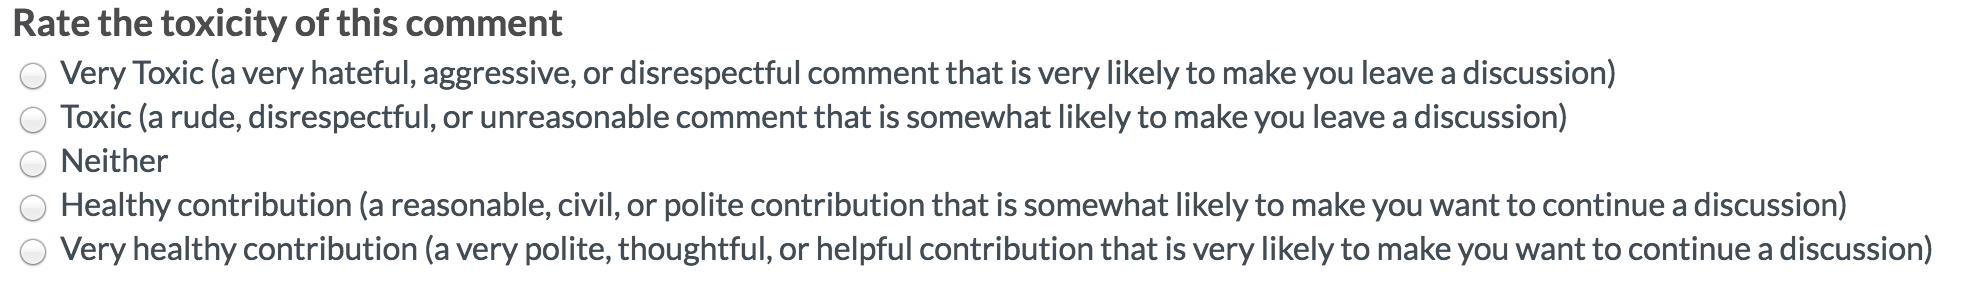
\includegraphics[width=\columnwidth]{figures/toxicity_question.png}
\caption{blah blah}\label{fig:method}
\end{center}
\end{figure}


% Bibliography
\bibliographystyle{ACM-Reference-Format}
\bibliography{acmsmall-sample-bibfile,websci-2017}

\medskip


\end{document}
% End of v2-acmsmall-sample.tex (March 2012) - Gerry Murray, ACM


